\section{Example Chapter}

Lorem ipsum dolor sit amet, consectetuer adipiscing elit. Donec odio. Quisque volutpat mattis eros. Nullam malesuada erat ut turpis. Suspendisse urna nibh, viverra non, semper suscipit, posuere a, pede.

\begin{graybox}
  Hello World!~\parencite{einstein}
\end{graybox}

Praesent dapibus, neque id cursus faucibus, tortor neque egestas augue, eu vulputate magna eros eu erat. Aliquam erat volutpat. Nam dui mi, tincidunt quis, accumsan porttitor, facilisis luctus, metus.

\begin{figure}
  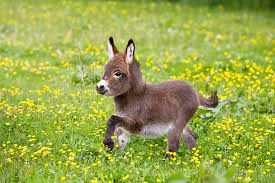
\includegraphics[width=7cm]{inc/donkey.jpg}
  \caption{Donkey}
\end{figure}

Phasellus ultrices nulla quis nibh. Quisque a lectus. Donec consectetuer ligula vulputate sem tristique cursus. Nam nulla quam, gravida non, commodo a, sodales sit amet, nisi. \footnote{Make sure that all references from the list are cited in the text. Those not cited should be moved to a separate \textit{Further Reading} section or chapter.}

\begin{table}[!htp]
  \caption{Please write a table caption here}
  \label{tab:1}
  \begin{tabular*}{14.0cm}{p{2.0cm}p{2.5cm}p{2.0cm}p{7.5cm}}
    \toprule
    Classes & Subclass & Length & Action Mechanism  \\
    \midrule
    Translation & mRNA$^a$  & 22 (19--25) & Translation repression, mRNA cleavage\\
    Translation & mRNA cleavage & 21 & mRNA cleavage\\
    Translation & mRNA  & 21--22 & mRNA cleavage\\
    Translation & mRNA  & 24--26 & Histone and DNA Modification\\
    \bottomrule
  \end{tabular*}
  $^a$ Table foot note (with superscript)
\end{table}

Sed adipiscing ornare risus. Morbi est est, blandit sit amet, sagittis vel, euismod vel, velit. Pellentesque egestas sem. Suspendisse commodo ullamcorper magna~\parencite{knuthwebsite}.

\begin{figure}
  \begin{tikzpicture}[
  roundnode/.style={%
    circle,%
    %draw=RoyalBlue,
    draw=black,
    %draw=green!60,%
    %fill=green!80,%
    %very thick,%
    thin,
    minimum size=5mm%
  },
  squarednode/.style={%
    rectangle,%
    %draw=red!60,%
    %fill=red!5,%
    draw=black,
    very thick,%
    minimum size=5mm%
  }
]

  \node [roundnode]   (n1) at (0.0,1.0) {N1};
  \node [squarednode] (n2) at (0.0,3.0) {N2};
  \node [roundnode]   (n3) at (5.0,2.0) {N3};
  \node [squarednode] (n4) at (13.0,4.0) {N4};
  \node [squarednode] (n5) at (8.0,1.5) {N5};

  \draw[latex-latex] (n1) -- (n2);
  \draw[latex-latex] (n1) -- (n3);
  \draw[latex-latex] (n3) -- (n4);
  \draw[latex-latex] (n3) -- (n5);

\end{tikzpicture}

  \caption{Tikz picture}
  \label{fig:tikz}
\end{figure}

\begin{figure}
    \centering
    \begin{ganttchart}[
    hgrid=false,
    vgrid={dotted},
    y unit title=0.3cm,
    y unit chart=0.37cm,
    title height = 1,
    x unit=4.3mm,
    bar height=0.7,
    group peaks width=0.08mm,
    group peaks height=0.08mm,
    group label font=\normalsize,
    milestone height=0.2mm,
    milestone top shift=0.15mm,
    milestone left shift=0.11mm,
    milestone right shift=-0.11mm,
    milestone inline label node/.append style={right=0.1mm}
    ]{1}{32}

      \gantttitle{Project}{32} \\
      \gantttitlelist{1,...,32}{1} \\

      \ganttbar{}{-20}{-19} \\

      \ganttgroup[inline]{\scriptsize{Algorithm Implementation}}{1}{24}\\
        \ganttbar[progress=37,inline]{\scriptsize{Plannning}}{1}{4} \\
        \ganttmilestone[inline]{\scriptsize{M 1}}{4} \\
        \ganttbar[inline]{\scriptsize{HurrDurr!}}{2}{6} \\
    \end{ganttchart}
    \caption{Project Plan}
    \label{fig:gantt}
\end{figure}
